\documentclass[a4paper,11pt]{article}
\usepackage[margin=19mm]{geometry}
\usepackage[T1]{fontenc}
\usepackage[utf8]{inputenc}
\usepackage[ngerman]{babel}
\usepackage{lmodern,graphicx,booktabs,pgfplots,enumitem}
\pgfplotsset{compat=1.18}
\definecolor{ochre}{RGB}{155,112,0}
\definecolor{navy}{RGB}{36,92,170}
\definecolor{brick}{RGB}{185,56,50}
\setlength{\parindent}{0pt}
\setlength{\parskip}{3pt}
\setlength{\tabcolsep}{5pt}
\renewcommand{\arraystretch}{1.06}
\setlength{\topsep}{3pt}
\raggedbottom
\setlist[itemize]{leftmargin=*,itemsep=3pt,topsep=4pt}
\begin{document}
\textbf{Test 1 -- Haus, CODED mit zwei Events (ohne Pinning)} \hfill \texttt{2026111301}

{\small Build bleE, CODED, 2 Events, Scannerlimit offen, Intervall Standard\par 5 Seiten à 32 Byte, 1 s Abstand, Normalbetrieb}

\begin{center}\begin{minipage}[c]{.43\linewidth}\centering
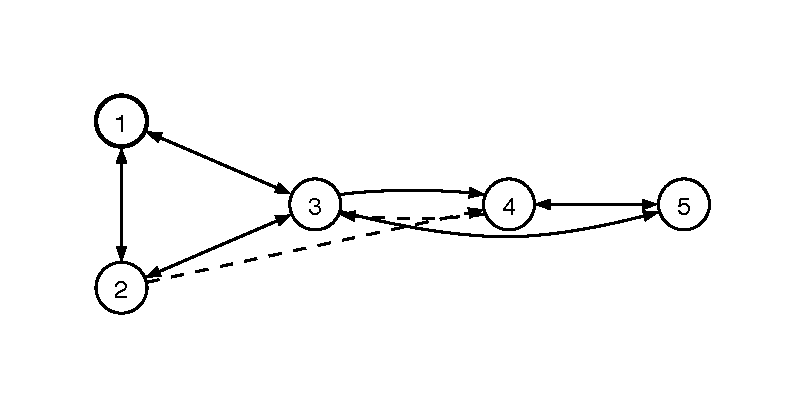
\includegraphics[width=\linewidth,height=3.5cm,keepaspectratio]{images/g1.pdf}
\end{minipage}\hfill\begin{minipage}[c]{.53\linewidth}
\begin{center}
\footnotesize
\begin{tabular}{c*{5}{r}}\toprule
S / E & 1 & 2 & 3 & 4 & 5 \\ \midrule
1 & -- & 60/6 & 41/3 & 0/0 & 0/0 \\
2 & 71/2 & -- & 47/3 & 6/0 & 0/0 \\
3 & 36/3 & 70/4 & -- & 13/2 & 2/1 \\
4 & 0/0 & 0/0 & 11/0 & -- & 40/2 \\
5 & 0/0 & 0/0 & 0/0 & 28/1 & -- \\
\bottomrule\end{tabular}
\end{center}
\end{minipage}\end{center}

{\small Pfeil vom Sender zum Empfänger\enspace\textbullet\enspace Durchgezogen bei Seitenframes\enspace\textbullet\enspace Gestrichelt bei Beacons allein\par Matrix über das ganze Log\enspace\textbullet\enspace Senderzeile, Empfängerspalte\enspace\textbullet\enspace Beacons/Seitenframes je Sequenz}

\begin{center}
\footnotesize
\begin{tabular}{crclrrrr}\toprule
Board & Lokal (s) & Seiten & IDs & RX & TX & Dup. & Bad \\ \midrule
1 & 420,0 & Quelle & 0, 1, 2, 3, 4 & 146 & 93 & 6 & 1 \\
2 & 420,0 & 5/5 & 0, 1, 2, 3, 4 & 208 & 91 & 6 & 0 \\
3 & 420,0 & 5/5 & 0, 1, 2, 3, 4 & 121 & 92 & 1 & 0 \\
4 & 420,0 & 3/5 & 0, 3, 4 & 60 & 91 & 0 & 0 \\
5 & 420,0 & 3/5 & 0, 3, 4 & 60 & 87 & 0 & 1 \\
\bottomrule\end{tabular}
\end{center}

\begin{center}\begin{tikzpicture}\begin{axis}[
width=16.2cm,height=5.4cm,xmin=0,xmax=300,ymin=-.12,ymax=5.55,
xtick={0,60,120,180,240,300},ytick={0,1,2,3,4,5},axis lines=left,grid=major,major grid style={gray!17},
xlabel={Sekunden seit Source-Start (geschätzt)},ylabel={Verschiedene Seiten},
tick label style={font=\footnotesize},label style={font=\footnotesize},
legend style={draw=none,font=\footnotesize,at={(.5,-.27)},anchor=north,legend columns=4}]
\addplot[ochre,dashdotted,thick,const plot,no marks] coordinates {(0.000,0) (0.177,1) (1.352,2) (3.240,3) (4.261,4) (19.390,5) (300.000,5)};
\addlegendentry{Board 2}
\addplot[navy,solid,thick,const plot,no marks] coordinates {(0.000,0) (0.176,1) (1.518,2) (3.391,3) (4.415,4) (19.402,5) (300.000,5)};
\addlegendentry{Board 3}
\addplot[brick,dashed,thick,const plot,no marks] coordinates {(0.000,0) (0.202,1) (4.431,2) (165.602,3) (300.000,3)};
\addlegendentry{Board 4}
\addplot[black,densely dotted,thick,const plot,no marks] coordinates {(0.000,0) (0.189,1) (58.531,2) (165.615,3) (300.000,3)};
\addlegendentry{Board 5}
\end{axis}\end{tikzpicture}\end{center}

\begin{center}
\footnotesize
\begin{tabular}{ccccc}\toprule
Seite & Board 2 & Board 3 & Board 4 & Board 5 \\ \midrule
0 & 10,767 (1) & 22,791 (1) & 33,755 (5) & 42,994 (3) \\
1 & 11,942 (1) & 24,133 (2) & fehlt & fehlt \\
2 & 29,980 (1) & 42,017 (2) & fehlt & fehlt \\
3 & 13,830 (1) & 26,006 (1) & 199,155 (3) & 208,420 (4) \\
4 & 14,851 (1) & 27,030 (1) & 37,984 (3) & 101,336 (4) \\
5/5 nach & 29,980 & 42,017 & -- & -- \\
\bottomrule\end{tabular}
\end{center}
\newpage
\textbf{Test 2 -- Haus, Ausgangsstand (ohne Pinning)} \hfill \texttt{2026111302}

{\small Build 9539f99, CODED, 1 Event, Scannerlimit 1, Intervall 50--100 ms\par 5 Seiten à 32 Byte, 1 s Abstand, Normalbetrieb}

\begin{center}\begin{minipage}[c]{.43\linewidth}\centering
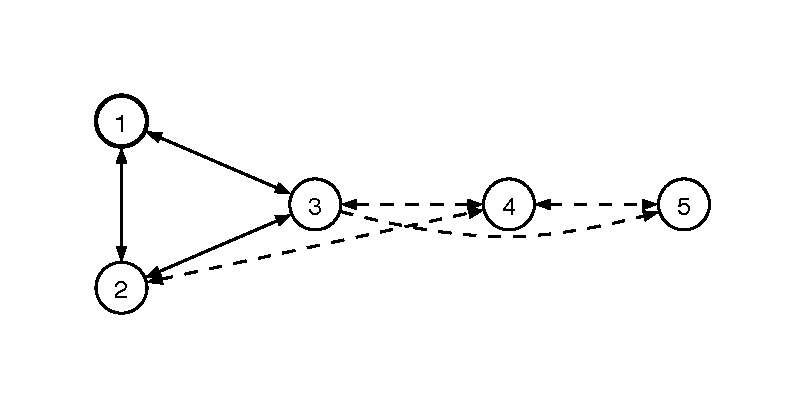
\includegraphics[width=\linewidth,height=3.5cm,keepaspectratio]{images/g2.pdf}
\end{minipage}\hfill\begin{minipage}[c]{.53\linewidth}
\begin{center}
\footnotesize
\begin{tabular}{c*{5}{r}}\toprule
S / E & 1 & 2 & 3 & 4 & 5 \\ \midrule
1 & -- & 51/4 & 3/1 & 0/0 & 0/0 \\
2 & 50/5 & -- & 43/5 & 8/0 & 0/0 \\
3 & 3/1 & 56/5 & -- & 7/0 & 3/0 \\
4 & 0/0 & 8/0 & 5/0 & -- & 25/0 \\
5 & 0/0 & 0/0 & 0/0 & 21/0 & -- \\
\bottomrule\end{tabular}
\end{center}
\end{minipage}\end{center}

{\small Pfeil vom Sender zum Empfänger\enspace\textbullet\enspace Durchgezogen bei Seitenframes\enspace\textbullet\enspace Gestrichelt bei Beacons allein\par Matrix über das ganze Log\enspace\textbullet\enspace Senderzeile, Empfängerspalte\enspace\textbullet\enspace Beacons/Seitenframes je Sequenz}

\begin{center}
\footnotesize
\begin{tabular}{crclrrrr}\toprule
Board & Lokal (s) & Seiten & IDs & RX & TX & Dup. & Bad \\ \midrule
1 & 420,0 & Quelle & 0, 1, 2, 3, 4 & 59 & 91 & 6 & 0 \\
2 & 420,0 & 5/5 & 0, 1, 2, 3, 4 & 124 & 93 & 4 & 0 \\
3 & 420,0 & 5/5 & 0, 1, 2, 3, 4 & 57 & 93 & 1 & 0 \\
4 & 420,0 & 0/5 & -- & 36 & 85 & 0 & 0 \\
5 & 420,0 & 0/5 & -- & 28 & 84 & 0 & 0 \\
\bottomrule\end{tabular}
\end{center}

\begin{center}\begin{tikzpicture}\begin{axis}[
width=16.2cm,height=5.4cm,xmin=0,xmax=300,ymin=-.12,ymax=5.55,
xtick={0,60,120,180,240,300},ytick={0,1,2,3,4,5},axis lines=left,grid=major,major grid style={gray!17},
xlabel={Sekunden seit Source-Start (geschätzt)},ylabel={Verschiedene Seiten},
tick label style={font=\footnotesize},label style={font=\footnotesize},
legend style={draw=none,font=\footnotesize,at={(.5,-.27)},anchor=north,legend columns=4}]
\addplot[ochre,dashdotted,thick,const plot,no marks] coordinates {(0.000,0) (0.046,1) (1.055,2) (2.076,3) (3.096,4) (4.117,5) (300.000,5)};
\addlegendentry{Board 2}
\addplot[navy,solid,thick,const plot,no marks] coordinates {(0.000,0) (0.033,1) (1.866,2) (2.088,3) (3.109,4) (6.635,5) (300.000,5)};
\addlegendentry{Board 3}
\addplot[brick,dashed,thick,const plot,no marks] coordinates {(0.000,0) (300.000,0)};
\addlegendentry{Board 4}
\addplot[black,densely dotted,thick,const plot,no marks] coordinates {(0.000,0) (300.000,0)};
\addlegendentry{Board 5}
\end{axis}\end{tikzpicture}\end{center}

\begin{center}
\footnotesize
\begin{tabular}{ccccc}\toprule
Seite & Board 2 & Board 3 & Board 4 & Board 5 \\ \midrule
0 & 9,253 (3) & 23,447 (1) & fehlt & fehlt \\
1 & 10,262 (1) & 25,280 (2) & fehlt & fehlt \\
2 & 11,283 (1) & 25,502 (2) & fehlt & fehlt \\
3 & 12,303 (1) & 26,523 (2) & fehlt & fehlt \\
4 & 13,324 (1) & 30,049 (2) & fehlt & fehlt \\
5/5 nach & 13,324 & 30,049 & -- & -- \\
\bottomrule\end{tabular}
\end{center}
\newpage
\textbf{Test 3 -- Haus, Wechsel auf 1M (ohne Pinning)} \hfill \texttt{2026111303}

{\small Build bleD, 1M, 2 Events, Scannerlimit offen, Intervall Standard\par 5 Seiten à 32 Byte, 1 s Abstand, Normalbetrieb}

\begin{center}\begin{minipage}[c]{.43\linewidth}\centering
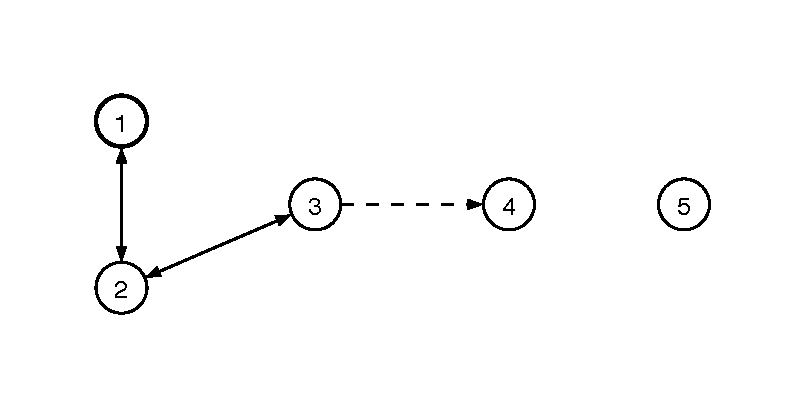
\includegraphics[width=\linewidth,height=3.5cm,keepaspectratio]{images/g3.pdf}
\end{minipage}\hfill\begin{minipage}[c]{.53\linewidth}
\begin{center}
\footnotesize
\begin{tabular}{c*{5}{r}}\toprule
S / E & 1 & 2 & 3 & 4 & 5 \\ \midrule
1 & -- & 59/6 & 0/0 & 0/0 & 0/0 \\
2 & 57/9 & -- & 30/6 & 0/0 & 0/0 \\
3 & 0/0 & 25/2 & -- & 5/0 & 0/0 \\
4 & 0/0 & 0/0 & 0/0 & -- & 0/0 \\
5 & 0/0 & 0/0 & 0/0 & 0/0 & -- \\
\bottomrule\end{tabular}
\end{center}
\end{minipage}\end{center}

{\small Pfeil vom Sender zum Empfänger\enspace\textbullet\enspace Durchgezogen bei Seitenframes\enspace\textbullet\enspace Gestrichelt bei Beacons allein\par Matrix über das ganze Log\enspace\textbullet\enspace Senderzeile, Empfängerspalte\enspace\textbullet\enspace Beacons/Seitenframes je Sequenz}

\begin{center}
\footnotesize
\begin{tabular}{crclrrrr}\toprule
Board & Lokal (s) & Seiten & IDs & RX & TX & Dup. & Bad \\ \midrule
1 & 420,0 & Quelle & 0, 1, 2, 3, 4 & 90 & 92 & 11 & 0 \\
2 & 420,0 & 5/5 & 0, 1, 2, 3, 4 & 122 & 99 & 3 & 0 \\
3 & 420,0 & 5/5 & 0, 1, 2, 3, 4 & 41 & 89 & 2 & 0 \\
4 & 420,0 & 0/5 & -- & 5 & 84 & 0 & 0 \\
5 & 420,0 & 0/5 & -- & 0 & 85 & 0 & 0 \\
\bottomrule\end{tabular}
\end{center}

\begin{center}\begin{tikzpicture}\begin{axis}[
width=16.2cm,height=5.4cm,xmin=0,xmax=420,ymin=-.12,ymax=5.55,
xtick={0,60,120,180,240,300,360,420},ytick={0,1,2,3,4,5},axis lines=left,grid=major,major grid style={gray!17},
xlabel={Sekunden seit jeweiligem Boardstart},ylabel={Verschiedene Seiten},
tick label style={font=\footnotesize},label style={font=\footnotesize},
legend style={draw=none,font=\footnotesize,at={(.5,-.27)},anchor=north,legend columns=4}]
\addplot[ochre,dashdotted,thick,const plot,no marks] coordinates {(0.000,0) (8.821,1) (10.002,2) (10.863,3) (11.884,4) (12.905,5) (420.000,5)};
\addlegendentry{Board 2}
\addplot[navy,solid,thick,const plot,no marks] coordinates {(0.000,0) (25.840,1) (85.827,2) (327.509,3) (336.791,4) (407.552,5) (420.000,5)};
\addlegendentry{Board 3}
\addplot[brick,dashed,thick,const plot,no marks] coordinates {(0.000,0) (420.000,0)};
\addlegendentry{Board 4}
\addplot[black,densely dotted,thick,const plot,no marks] coordinates {(0.000,0) (420.000,0)};
\addlegendentry{Board 5}
\end{axis}\end{tikzpicture}\end{center}

\begin{center}
\footnotesize
\begin{tabular}{ccccc}\toprule
Seite & Board 2 & Board 3 & Board 4 & Board 5 \\ \midrule
0 & 8,821 (1) & 25,840 (2) & fehlt & fehlt \\
1 & 10,002 (1) & 327,509 (2) & fehlt & fehlt \\
2 & 10,863 (1) & 336,791 (2) & fehlt & fehlt \\
3 & 11,884 (1) & 85,827 (2) & fehlt & fehlt \\
4 & 12,905 (1) & 407,552 (2) & fehlt & fehlt \\
5/5 nach & 12,905 & 407,552 & -- & -- \\
\bottomrule\end{tabular}
\end{center}
\newpage
\textbf{Test 4 -- Haus, Quellenstopp mit zwei Events (mit Pinning)} \hfill \texttt{2026111304}

{\small Build bleE, CODED, 2 Events, Scannerlimit offen, Intervall Standard\par 5 Seiten à 32 Byte, 1 s Abstand, Quelle gepinnt, Wiederholung alle 5 s, Stopp nach 184,881 s}

\begin{center}\begin{minipage}[c]{.43\linewidth}\centering
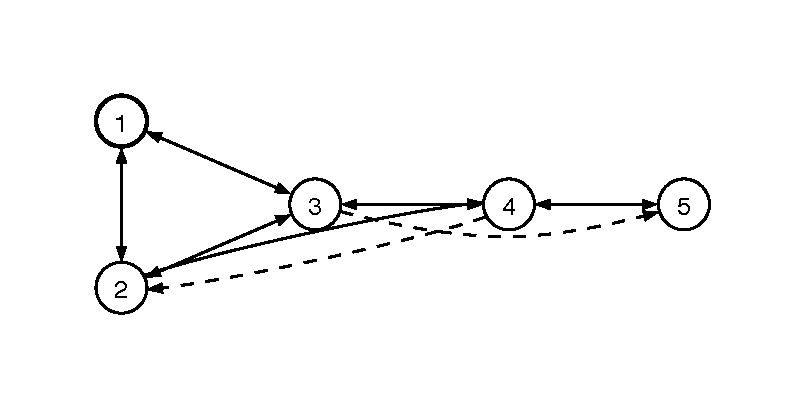
\includegraphics[width=\linewidth,height=3.5cm,keepaspectratio]{images/g4.pdf}
\end{minipage}\hfill\begin{minipage}[c]{.53\linewidth}
\begin{center}
\footnotesize
\begin{tabular}{c*{5}{r}}\toprule
S / E & 1 & 2 & 3 & 4 & 5 \\ \midrule
1 & -- & 28/53 & 16/28 & 0/0 & 0/0 \\
2 & 24/19 & -- & 81/9 & 4/2 & 0/0 \\
3 & 15/6 & 95/8 & -- & 88/14 & 6/0 \\
4 & 0/0 & 2/0 & 53/5 & -- & 35/7 \\
5 & 0/0 & 0/0 & 0/0 & 37/3 & -- \\
\bottomrule\end{tabular}
\end{center}
\end{minipage}\end{center}

{\small Pfeil vom Sender zum Empfänger\enspace\textbullet\enspace Durchgezogen bei Seitenframes\enspace\textbullet\enspace Gestrichelt bei Beacons allein\par Matrix über das ganze Log\enspace\textbullet\enspace Senderzeile, Empfängerspalte\enspace\textbullet\enspace Beacons/Seitenframes je Sequenz}

\begin{center}
\footnotesize
\begin{tabular}{crclrrrr}\toprule
Board & Lokal (s) & Seiten & IDs & RX & TX & Dup. & Bad \\ \midrule
1 & 184,9 & Quelle & 0, 1, 2, 3, 4 & 74 & 98 & 26 & 0 \\
2 & 900,0 & 5/5 & 0, 1, 2, 3, 4 & 234 & 217 & 67 & 0 \\
3 & 900,0 & 5/5 & 0, 1, 2, 3, 4 & 213 & 218 & 38 & 0 \\
4 & 900,0 & 5/5 & 0, 1, 2, 3, 4 & 169 & 210 & 14 & 1 \\
5 & 300,0 & 5/5 & 0, 1, 2, 3, 4 & 60 & 66 & 3 & 0 \\
\bottomrule\end{tabular}
\end{center}

\begin{center}\begin{tikzpicture}\begin{axis}[
width=16.2cm,height=5.4cm,xmin=0,xmax=540,ymin=-.12,ymax=5.55,
xtick={0,100,200,300,400,500},ytick={0,1,2,3,4,5},axis lines=left,grid=major,major grid style={gray!17},
xlabel={Sekunden seit Source-Start (geschätzt)},ylabel={Verschiedene Seiten},
tick label style={font=\footnotesize},label style={font=\footnotesize},
legend style={draw=none,font=\footnotesize,at={(.5,-.27)},anchor=north,legend columns=4}]
\addplot[ochre,dashdotted,thick,const plot,no marks] coordinates {(0.000,0) (0.705,1) (2.038,2) (3.217,3) (4.243,4) (14.278,5) (540.000,5)};
\addlegendentry{Board 2}
\addplot[navy,solid,thick,const plot,no marks] coordinates {(0.000,0) (0.670,1) (3.194,2) (4.025,3) (4.207,4) (14.242,5) (540.000,5)};
\addlegendentry{Board 3}
\addplot[brick,dashed,thick,const plot,no marks] coordinates {(0.000,0) (4.421,1) (39.434,2) (49.477,3) (54.498,4) (59.528,5) (540.000,5)};
\addlegendentry{Board 4}
\addplot[black,densely dotted,thick,const plot,no marks] coordinates {(239.356,0) (338.426,1) (363.550,2) (368.793,3) (378.896,4) (482.997,5) (539.356,5)};
\addlegendentry{Board 5}
\draw[gray,densely dashed] (axis cs:184.881,0) -- (axis cs:184.881,5.5);
\node[font=\scriptsize,fill=white,inner sep=1pt] at (axis cs:184.881,.65) {Stopp 1};
\draw[gray,densely dashed] (axis cs:239.356,0) -- (axis cs:239.356,5.5);
\node[font=\scriptsize,fill=white,inner sep=1pt] at (axis cs:239.356,.65) {Start 5};
\end{axis}\end{tikzpicture}\end{center}

\begin{center}
\footnotesize
\begin{tabular}{ccccc}\toprule
Seite & Board 2 & Board 3 & Board 4 & Board 5 \\ \midrule
0 & 14,909 (1) & 26,809 (1) & 97,408 (3) & 124,194 (4) \\
1 & 28,482 (1) & 40,381 (1) & 77,314 (3) & 129,437 (4) \\
2 & 16,242 (1) & 30,164 (2) & 42,301 (3) & 139,540 (4) \\
3 & 17,421 (1) & 29,333 (2) & 87,357 (3) & 99,070 (4) \\
4 & 18,447 (1) & 30,346 (1) & 92,378 (2) & 243,641 (4) \\
5/5 nach & 28,482 & 40,381 & 97,408 & 243,641 \\
\bottomrule\end{tabular}
\end{center}
\newpage
\textbf{Test 5 -- Haus, Quellenstopp im Ausgangsstand (mit Pinning)} \hfill \texttt{2026111305}

{\small Build 9539f99, CODED, 1 Event, Scannerlimit 1, Intervall 50--100 ms\par 5 Seiten à 32 Byte, 1 s Abstand, Quelle gepinnt, Wiederholung alle 5 s, Stopp nach 183,807 s}

\begin{center}\begin{minipage}[c]{.43\linewidth}\centering
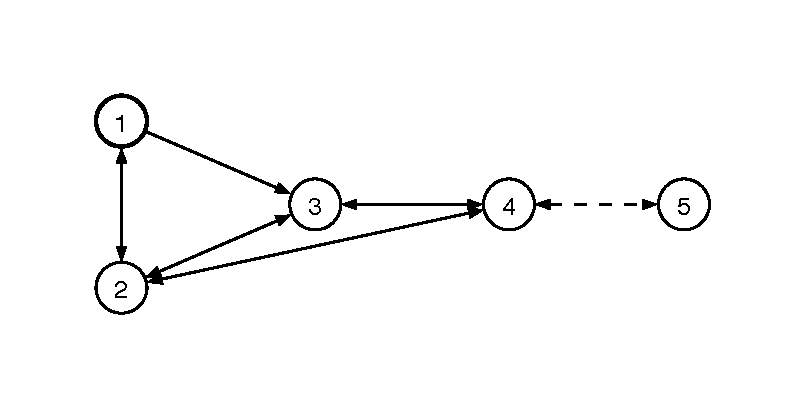
\includegraphics[width=\linewidth,height=3.5cm,keepaspectratio]{images/g5.pdf}
\end{minipage}\hfill\begin{minipage}[c]{.53\linewidth}
\begin{center}
\footnotesize
\begin{tabular}{c*{5}{r}}\toprule
S / E & 1 & 2 & 3 & 4 & 5 \\ \midrule
1 & -- & 29/38 & 0/5 & 0/0 & 0/0 \\
2 & 19/22 & -- & 79/15 & 16/8 & 0/0 \\
3 & 0/0 & 114/5 & -- & 35/3 & 0/0 \\
4 & 0/0 & 11/1 & 30/1 & -- & 19/0 \\
5 & 0/0 & 0/0 & 0/0 & 11/0 & -- \\
\bottomrule\end{tabular}
\end{center}
\end{minipage}\end{center}

{\small Pfeil vom Sender zum Empfänger\enspace\textbullet\enspace Durchgezogen bei Seitenframes\enspace\textbullet\enspace Gestrichelt bei Beacons allein\par Matrix über das ganze Log\enspace\textbullet\enspace Senderzeile, Empfängerspalte\enspace\textbullet\enspace Beacons/Seitenframes je Sequenz}

\begin{center}
\footnotesize
\begin{tabular}{crclrrrr}\toprule
Board & Lokal (s) & Seiten & IDs & RX & TX & Dup. & Bad \\ \midrule
1 & 183,8 & Quelle & 0, 1, 2, 3, 4 & 41 & 98 & 22 & 0 \\
2 & 900,0 & 5/5 & 0, 1, 2, 3, 4 & 198 & 211 & 39 & 0 \\
3 & 900,0 & 5/5 & 0, 1, 2, 3, 4 & 130 & 203 & 16 & 0 \\
4 & 900,0 & 5/5 & 0, 1, 2, 3, 4 & 73 & 193 & 6 & 0 \\
5 & 300,0 & 0/5 & -- & 19 & 61 & 0 & 0 \\
\bottomrule\end{tabular}
\end{center}

\begin{center}\begin{tikzpicture}\begin{axis}[
width=16.2cm,height=5.4cm,xmin=0,xmax=560,ymin=-.12,ymax=5.55,
xtick={0,100,200,300,400,500},ytick={0,1,2,3,4,5},axis lines=left,grid=major,major grid style={gray!17},
xlabel={Sekunden seit Source-Start (geschätzt)},ylabel={Verschiedene Seiten},
tick label style={font=\footnotesize},label style={font=\footnotesize},
legend style={draw=none,font=\footnotesize,at={(.5,-.27)},anchor=north,legend columns=4}]
\addplot[ochre,dashdotted,thick,const plot,no marks] coordinates {(0.000,0) (2.054,1) (4.096,2) (14.138,3) (23.214,4) (37.851,5) (560.000,5)};
\addlegendentry{Board 2}
\addplot[navy,solid,thick,const plot,no marks] coordinates {(0.000,0) (2.053,1) (14.150,2) (18.491,3) (34.221,4) (73.537,5) (560.000,5)};
\addlegendentry{Board 3}
\addplot[brick,dashed,thick,const plot,no marks] coordinates {(0.000,0) (14.152,1) (19.172,2) (54.318,3) (96.004,4) (124.613,5) (560.000,5)};
\addlegendentry{Board 4}
\addplot[black,densely dotted,thick,const plot,no marks] coordinates {(258.299,0) (558.299,0)};
\addlegendentry{Board 5}
\draw[gray,densely dashed] (axis cs:183.807,0) -- (axis cs:183.807,5.5);
\node[font=\scriptsize,fill=white,inner sep=1pt] at (axis cs:183.807,.65) {Stopp 1};
\draw[gray,densely dashed] (axis cs:258.299,0) -- (axis cs:258.299,5.5);
\node[font=\scriptsize,fill=white,inner sep=1pt] at (axis cs:258.299,.65) {Start 5};
\end{axis}\end{tikzpicture}\end{center}

\begin{center}
\footnotesize
\begin{tabular}{ccccc}\toprule
Seite & Board 2 & Board 3 & Board 4 & Board 5 \\ \midrule
0 & 49,986 (1) & 60,413 (1) & 134,906 (2) & fehlt \\
1 & 26,273 (1) & 40,342 (2) & 53,054 (2) & fehlt \\
2 & 14,189 (1) & 28,245 (1) & 58,074 (3) & fehlt \\
3 & 35,349 (1) & 99,729 (2) & 163,515 (2) & fehlt \\
4 & 16,231 (1) & 44,683 (2) & 93,220 (2) & fehlt \\
5/5 nach & 49,986 & 99,729 & 163,515 & -- \\
\bottomrule\end{tabular}
\end{center}
\newpage
\textbf{Test 6 -- Hub, Ausgangsstand (ohne Pinning)} \hfill \texttt{2026111306}

{\small Build 9539f99, CODED, 1 Event, Scannerlimit 1, Intervall 50--100 ms\par 5 Seiten à 32 Byte, 1 s Abstand, Normalbetrieb}

\begin{center}\begin{minipage}[c]{.43\linewidth}\centering
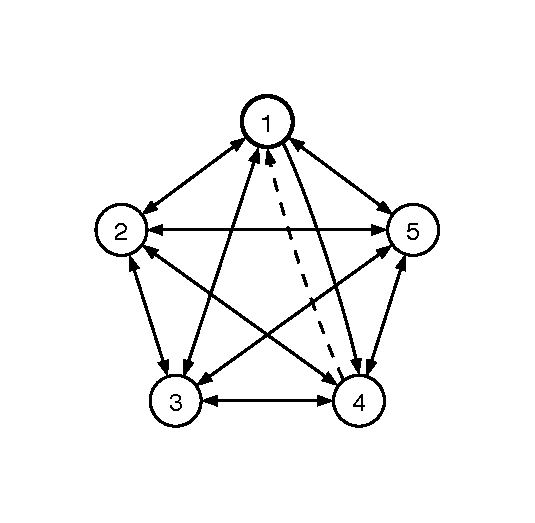
\includegraphics[width=\linewidth,height=3.5cm,keepaspectratio]{images/g6.pdf}
\end{minipage}\hfill\begin{minipage}[c]{.53\linewidth}
\begin{center}
\footnotesize
\begin{tabular}{c*{5}{r}}\toprule
S / E & 1 & 2 & 3 & 4 & 5 \\ \midrule
1 & -- & 38/5 & 34/4 & 36/2 & 41/3 \\
2 & 49/5 & -- & 45/3 & 40/5 & 47/5 \\
3 & 45/1 & 39/1 & -- & 48/1 & 42/1 \\
4 & 38/0 & 43/3 & 45/2 & -- & 39/1 \\
5 & 45/3 & 42/3 & 47/2 & 44/2 & -- \\
\bottomrule\end{tabular}
\end{center}
\end{minipage}\end{center}

{\small Pfeil vom Sender zum Empfänger\enspace\textbullet\enspace Durchgezogen bei Seitenframes\enspace\textbullet\enspace Gestrichelt bei Beacons allein\par Matrix über das ganze Log\enspace\textbullet\enspace Senderzeile, Empfängerspalte\enspace\textbullet\enspace Beacons/Seitenframes je Sequenz}

\begin{center}
\footnotesize
\begin{tabular}{crclrrrr}\toprule
Board & Lokal (s) & Seiten & IDs & RX & TX & Dup. & Bad \\ \midrule
1 & 300,0 & Quelle & 0, 1, 2, 3, 4 & 186 & 70 & 9 & 0 \\
2 & 300,0 & 5/5 & 0, 1, 2, 3, 4 & 174 & 70 & 7 & 0 \\
3 & 300,0 & 5/5 & 0, 1, 2, 3, 4 & 182 & 67 & 6 & 0 \\
4 & 300,0 & 5/5 & 0, 1, 2, 3, 4 & 178 & 67 & 5 & 0 \\
5 & 300,0 & 5/5 & 0, 1, 2, 3, 4 & 179 & 66 & 5 & 0 \\
\bottomrule\end{tabular}
\end{center}

\begin{center}\begin{tikzpicture}\begin{axis}[
width=16.2cm,height=5.4cm,xmin=0,xmax=25,ymin=-.12,ymax=5.55,
xtick={0,5,10,15,20,25},ytick={0,1,2,3,4,5},axis lines=left,grid=major,major grid style={gray!17},
xlabel={Sekunden seit Source-Start (geschätzt)},ylabel={Verschiedene Seiten},
tick label style={font=\footnotesize},label style={font=\footnotesize},
legend style={draw=none,font=\footnotesize,at={(.5,-.27)},anchor=north,legend columns=4}]
\addplot[ochre,dashdotted,thick,const plot,no marks] coordinates {(0.000,0) (0.011,1) (2.053,2) (3.074,3) (4.095,4) (19.282,5) (25.000,5)};
\addlegendentry{Board 2}
\addplot[navy,solid,thick,const plot,no marks] coordinates {(0.000,0) (2.053,1) (3.073,2) (4.106,3) (9.169,4) (19.269,5) (25.000,5)};
\addlegendentry{Board 3}
\addplot[brick,dashed,thick,const plot,no marks] coordinates {(0.000,0) (0.012,1) (2.054,2) (4.107,3) (14.467,4) (19.295,5) (25.000,5)};
\addlegendentry{Board 4}
\addplot[black,densely dotted,thick,const plot,no marks] coordinates {(0.000,0) (3.074,1) (4.212,2) (4.464,3) (9.607,4) (19.269,5) (25.000,5)};
\addlegendentry{Board 5}
\end{axis}\end{tikzpicture}\end{center}

\begin{center}
\footnotesize
\begin{tabular}{ccccc}\toprule
Seite & Board 2 & Board 3 & Board 4 & Board 5 \\ \midrule
0 & 0,062 (1) & 9,241 (4) & 0,102 (1) & 4,323 (2) \\
1 & 19,333 (5) & 19,341 (1) & 19,385 (2) & 19,380 (1) \\
2 & 2,104 (1) & 2,125 (1) & 2,144 (1) & 4,575 (2) \\
3 & 3,125 (1) & 3,145 (1) & 14,557 (2) & 3,185 (1) \\
4 & 4,146 (1) & 4,178 (2) & 4,197 (2) & 9,718 (3) \\
5/5 nach & 19,333 & 19,341 & 19,385 & 19,380 \\
\bottomrule\end{tabular}
\end{center}
\newpage
\textbf{Test 7 -- Hub, Scannerlimit entfernt (ohne Pinning)} \hfill \texttt{2026111307}

{\small Build bleB, CODED, 1 Event, Scannerlimit offen, Intervall 50--100 ms\par 5 Seiten à 32 Byte, 1 s Abstand, Normalbetrieb}

\begin{center}\begin{minipage}[c]{.43\linewidth}\centering
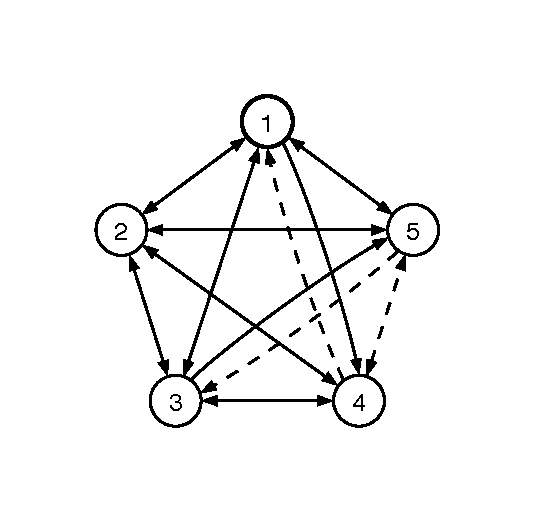
\includegraphics[width=\linewidth,height=3.5cm,keepaspectratio]{images/g7.pdf}
\end{minipage}\hfill\begin{minipage}[c]{.53\linewidth}
\begin{center}
\footnotesize
\begin{tabular}{c*{5}{r}}\toprule
S / E & 1 & 2 & 3 & 4 & 5 \\ \midrule
1 & -- & 33/2 & 33/4 & 36/4 & 47/5 \\
2 & 30/3 & -- & 40/2 & 39/2 & 36/3 \\
3 & 46/2 & 47/2 & -- & 51/1 & 46/1 \\
4 & 39/0 & 40/1 & 44/2 & -- & 46/0 \\
5 & 42/1 & 39/1 & 40/0 & 46/0 & -- \\
\bottomrule\end{tabular}
\end{center}
\end{minipage}\end{center}

{\small Pfeil vom Sender zum Empfänger\enspace\textbullet\enspace Durchgezogen bei Seitenframes\enspace\textbullet\enspace Gestrichelt bei Beacons allein\par Matrix über das ganze Log\enspace\textbullet\enspace Senderzeile, Empfängerspalte\enspace\textbullet\enspace Beacons/Seitenframes je Sequenz}

\begin{center}
\footnotesize
\begin{tabular}{crclrrrr}\toprule
Board & Lokal (s) & Seiten & IDs & RX & TX & Dup. & Bad \\ \midrule
1 & 300,0 & Quelle & 0, 1, 2, 3, 4 & 163 & 66 & 6 & 0 \\
2 & 300,0 & 5/5 & 0, 1, 2, 3, 4 & 165 & 65 & 1 & 0 \\
3 & 300,0 & 5/5 & 0, 1, 2, 3, 4 & 165 & 65 & 3 & 0 \\
4 & 300,0 & 5/5 & 0, 1, 2, 3, 4 & 179 & 64 & 2 & 0 \\
5 & 300,0 & 5/5 & 0, 1, 2, 3, 4 & 184 & 64 & 4 & 0 \\
\bottomrule\end{tabular}
\end{center}

\begin{center}\begin{tikzpicture}\begin{axis}[
width=16.2cm,height=5.4cm,xmin=0,xmax=25,ymin=-.12,ymax=5.55,
xtick={0,5,10,15,20,25},ytick={0,1,2,3,4,5},axis lines=left,grid=major,major grid style={gray!17},
xlabel={Sekunden seit Source-Start (geschätzt)},ylabel={Verschiedene Seiten},
tick label style={font=\footnotesize},label style={font=\footnotesize},
legend style={draw=none,font=\footnotesize,at={(.5,-.27)},anchor=north,legend columns=4}]
\addplot[ochre,dashdotted,thick,const plot,no marks] coordinates {(0.000,0) (1.057,1) (2.064,2) (3.074,3) (4.094,4) (4.578,5) (25.000,5)};
\addlegendentry{Board 2}
\addplot[navy,solid,thick,const plot,no marks] coordinates {(0.000,0) (1.045,1) (2.053,2) (3.074,3) (4.095,4) (4.558,5) (25.000,5)};
\addlegendentry{Board 3}
\addplot[brick,dashed,thick,const plot,no marks] coordinates {(0.000,0) (1.033,1) (2.053,2) (3.074,3) (4.095,4) (4.592,5) (25.000,5)};
\addlegendentry{Board 4}
\addplot[black,densely dotted,thick,const plot,no marks] coordinates {(0.000,0) (1.032,1) (2.053,2) (3.074,3) (4.095,4) (4.557,5) (25.000,5)};
\addlegendentry{Board 5}
\end{axis}\end{tikzpicture}\end{center}

\begin{center}
\footnotesize
\begin{tabular}{ccccc}\toprule
Seite & Board 2 & Board 3 & Board 4 & Board 5 \\ \midrule
0 & 4,647 (3) & 4,650 (1) & 4,708 (2) & 4,697 (1) \\
1 & 1,126 (3) & 1,137 (4) & 1,149 (1) & 1,172 (1) \\
2 & 2,133 (5) & 2,145 (1) & 2,169 (1) & 2,193 (1) \\
3 & 3,143 (1) & 3,166 (1) & 3,190 (1) & 3,214 (1) \\
4 & 4,163 (1) & 4,187 (1) & 4,211 (1) & 4,235 (1) \\
5/5 nach & 4,647 & 4,650 & 4,708 & 4,697 \\
\bottomrule\end{tabular}
\end{center}
\newpage
\textbf{Test 8 -- Hub, zweites Sendeevent (ohne Pinning)} \hfill \texttt{2026111308}

{\small Build bleF, CODED, 2 Events, Scannerlimit offen, Intervall 50--100 ms\par 5 Seiten à 32 Byte, 1 s Abstand, Normalbetrieb}

\begin{center}\begin{minipage}[c]{.43\linewidth}\centering
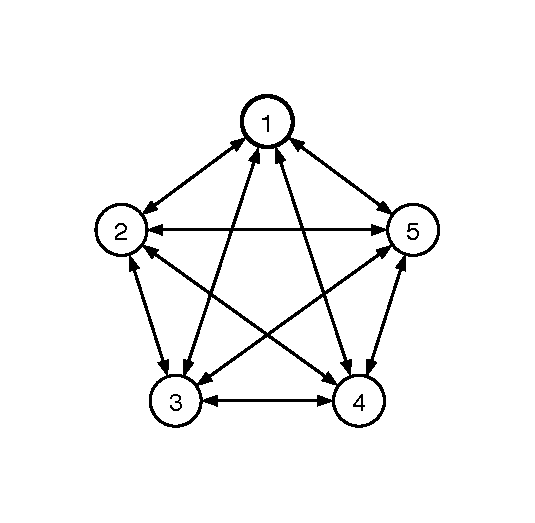
\includegraphics[width=\linewidth,height=3.5cm,keepaspectratio]{images/g8.pdf}
\end{minipage}\hfill\begin{minipage}[c]{.53\linewidth}
\begin{center}
\footnotesize
\begin{tabular}{c*{5}{r}}\toprule
S / E & 1 & 2 & 3 & 4 & 5 \\ \midrule
1 & -- & 48/1 & 50/3 & 44/4 & 54/3 \\
2 & 52/2 & -- & 50/2 & 54/3 & 49/2 \\
3 & 55/2 & 54/2 & -- & 54/2 & 55/2 \\
4 & 48/3 & 54/2 & 50/1 & -- & 57/3 \\
5 & 59/2 & 59/1 & 56/2 & 56/1 & -- \\
\bottomrule\end{tabular}
\end{center}
\end{minipage}\end{center}

{\small Pfeil vom Sender zum Empfänger\enspace\textbullet\enspace Durchgezogen bei Seitenframes\enspace\textbullet\enspace Gestrichelt bei Beacons allein\par Matrix über das ganze Log\enspace\textbullet\enspace Senderzeile, Empfängerspalte\enspace\textbullet\enspace Beacons/Seitenframes je Sequenz}

\begin{center}
\footnotesize
\begin{tabular}{crclrrrr}\toprule
Board & Lokal (s) & Seiten & IDs & RX & TX & Dup. & Bad \\ \midrule
1 & 300,0 & Quelle & 0, 1, 2, 3, 4 & 333 & 65 & 10 & 0 \\
2 & 300,0 & 5/5 & 0, 1, 2, 3, 4 & 337 & 65 & 1 & 0 \\
3 & 300,0 & 5/5 & 0, 1, 2, 3, 4 & 318 & 65 & 4 & 3 \\
4 & 300,0 & 5/5 & 0, 1, 2, 3, 4 & 321 & 64 & 7 & 1 \\
5 & 300,0 & 5/5 & 0, 1, 2, 3, 4 & 335 & 65 & 5 & 0 \\
\bottomrule\end{tabular}
\end{center}

\begin{center}\begin{tikzpicture}\begin{axis}[
width=16.2cm,height=5.4cm,xmin=0,xmax=25,ymin=-.12,ymax=5.55,
xtick={0,5,10,15,20,25},ytick={0,1,2,3,4,5},axis lines=left,grid=major,major grid style={gray!17},
xlabel={Sekunden seit Source-Start (geschätzt)},ylabel={Verschiedene Seiten},
tick label style={font=\footnotesize},label style={font=\footnotesize},
legend style={draw=none,font=\footnotesize,at={(.5,-.27)},anchor=north,legend columns=4}]
\addplot[ochre,dashdotted,thick,const plot,no marks] coordinates {(0.000,0) (0.023,1) (1.045,2) (2.053,3) (3.100,4) (4.212,5) (25.000,5)};
\addlegendentry{Board 2}
\addplot[navy,solid,thick,const plot,no marks] coordinates {(0.000,0) (0.124,1) (1.032,2) (2.066,3) (3.183,4) (4.095,5) (25.000,5)};
\addlegendentry{Board 3}
\addplot[brick,dashed,thick,const plot,no marks] coordinates {(0.000,0) (0.011,1) (1.032,2) (2.065,3) (3.074,4) (4.095,5) (25.000,5)};
\addlegendentry{Board 4}
\addplot[black,densely dotted,thick,const plot,no marks] coordinates {(0.000,0) (0.023,1) (1.032,2) (2.053,3) (3.087,4) (4.208,5) (25.000,5)};
\addlegendentry{Board 5}
\end{axis}\end{tikzpicture}\end{center}

\begin{center}
\footnotesize
\begin{tabular}{ccccc}\toprule
Seite & Board 2 & Board 3 & Board 4 & Board 5 \\ \midrule
0 & 0,074 (4) & 0,200 (4) & 0,110 (1) & 0,142 (4) \\
1 & 1,096 (4) & 1,108 (1) & 1,131 (1) & 1,151 (1) \\
2 & 2,104 (1) & 2,142 (5) & 2,164 (2) & 2,172 (1) \\
3 & 3,151 (5) & 3,259 (1) & 3,173 (1) & 3,206 (4) \\
4 & 4,263 (3) & 4,171 (1) & 4,194 (1) & 4,327 (1) \\
5/5 nach & 4,263 & 4,171 & 4,194 & 4,327 \\
\bottomrule\end{tabular}
\end{center}
\newpage
\textbf{Test 9 -- Hub, Standardintervalle (ohne Pinning)} \hfill \texttt{2026111309}

{\small Build bleE, CODED, 2 Events, Scannerlimit offen, Intervall Standard\par 5 Seiten à 32 Byte, 1 s Abstand, Normalbetrieb}

\begin{center}\begin{minipage}[c]{.43\linewidth}\centering
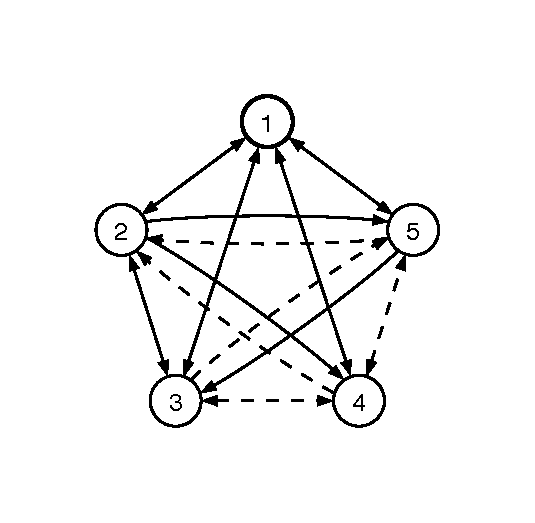
\includegraphics[width=\linewidth,height=3.5cm,keepaspectratio]{images/g9.pdf}
\end{minipage}\hfill\begin{minipage}[c]{.53\linewidth}
\begin{center}
\footnotesize
\begin{tabular}{c*{5}{r}}\toprule
S / E & 1 & 2 & 3 & 4 & 5 \\ \midrule
1 & -- & 49/4 & 47/5 & 49/5 & 48/5 \\
2 & 49/1 & -- & 48/1 & 48/2 & 51/1 \\
3 & 49/1 & 55/1 & -- & 53/0 & 53/0 \\
4 & 50/1 & 55/0 & 52/0 & -- & 55/0 \\
5 & 58/1 & 58/0 & 55/1 & 49/0 & -- \\
\bottomrule\end{tabular}
\end{center}
\end{minipage}\end{center}

{\small Pfeil vom Sender zum Empfänger\enspace\textbullet\enspace Durchgezogen bei Seitenframes\enspace\textbullet\enspace Gestrichelt bei Beacons allein\par Matrix über das ganze Log\enspace\textbullet\enspace Senderzeile, Empfängerspalte\enspace\textbullet\enspace Beacons/Seitenframes je Sequenz}

\begin{center}
\footnotesize
\begin{tabular}{crclrrrr}\toprule
Board & Lokal (s) & Seiten & IDs & RX & TX & Dup. & Bad \\ \midrule
1 & 300,0 & Quelle & 0, 1, 2, 3, 4 & 313 & 65 & 4 & 0 \\
2 & 300,0 & 5/5 & 0, 1, 2, 3, 4 & 343 & 64 & 0 & 0 \\
3 & 300,0 & 5/5 & 0, 1, 2, 3, 4 & 301 & 64 & 2 & 0 \\
4 & 300,0 & 5/5 & 0, 1, 2, 3, 4 & 304 & 64 & 2 & 0 \\
5 & 300,0 & 5/5 & 0, 1, 2, 3, 4 & 319 & 65 & 1 & 0 \\
\bottomrule\end{tabular}
\end{center}

\begin{center}\begin{tikzpicture}\begin{axis}[
width=16.2cm,height=5.4cm,xmin=0,xmax=25,ymin=-.12,ymax=5.55,
xtick={0,5,10,15,20,25},ytick={0,1,2,3,4,5},axis lines=left,grid=major,major grid style={gray!17},
xlabel={Sekunden seit Source-Start (geschätzt)},ylabel={Verschiedene Seiten},
tick label style={font=\footnotesize},label style={font=\footnotesize},
legend style={draw=none,font=\footnotesize,at={(.5,-.27)},anchor=north,legend columns=4}]
\addplot[ochre,dashdotted,thick,const plot,no marks] coordinates {(0.000,0) (0.011,1) (1.186,2) (2.054,3) (3.239,4) (4.096,5) (25.000,5)};
\addlegendentry{Board 2}
\addplot[navy,solid,thick,const plot,no marks] coordinates {(0.000,0) (0.012,1) (1.033,2) (2.054,3) (3.075,4) (4.096,5) (25.000,5)};
\addlegendentry{Board 3}
\addplot[brick,dashed,thick,const plot,no marks] coordinates {(0.000,0) (0.012,1) (1.034,2) (2.055,3) (3.076,4) (4.097,5) (25.000,5)};
\addlegendentry{Board 4}
\addplot[black,densely dotted,thick,const plot,no marks] coordinates {(0.000,0) (0.012,1) (1.187,2) (2.054,3) (3.075,4) (4.096,5) (25.000,5)};
\addlegendentry{Board 5}
\end{axis}\end{tikzpicture}\end{center}

\begin{center}
\footnotesize
\begin{tabular}{ccccc}\toprule
Seite & Board 2 & Board 3 & Board 4 & Board 5 \\ \midrule
0 & 0,062 (1) & 0,086 (1) & 0,109 (1) & 0,133 (1) \\
1 & 1,237 (1) & 1,107 (1) & 1,131 (1) & 1,308 (1) \\
2 & 2,105 (1) & 2,128 (1) & 2,152 (1) & 2,175 (1) \\
3 & 3,290 (3) & 3,149 (1) & 3,173 (1) & 3,196 (1) \\
4 & 4,147 (1) & 4,170 (1) & 4,194 (1) & 4,217 (1) \\
5/5 nach & 4,147 & 4,170 & 4,194 & 4,217 \\
\bottomrule\end{tabular}
\end{center}
\newpage
\textbf{Vergleich am Hub}

\begin{center}
\small
\begin{tabular}{lrrrrr}\toprule
Test & Lauf-ID & Median & Eindeutig & Roh & Alle 5/5 (s) \\ \midrule
Test 6 & 2026111306 & 0,71 & 899 & 899 & 19,3 \\
Test 7 & 2026111307 & 0,69 & 856 & 856 & 4,6 \\
Test 8 & 2026111308 & 0,87 & 1101 & 1644 & 4,2 \\
Test 9 & 2026111309 & 0,85 & 1060 & 1580 & 4,1 \\
\bottomrule\end{tabular}
\end{center}

{\small Median über 20 gerichtete Kontakte\enspace\textbullet\enspace Anteil gehörter Sequenzen von der ersten bis zur letzten gehörten Sequenz\par Verluste ausserhalb des Sequenzbereichs unberücksichtigt\enspace\textbullet\enspace Zeit bis 5/5 geschätzt ab Quellenstart}

\begin{center}
\small
\begin{tabular}{llrr}\toprule
Tests & Änderung & Kontakte besser & Median der Differenzen \\ \midrule
6 $\to$ 7 & Scannerlimit entfernt & 10/20 & 0,00 \\
7 $\to$ 8 & Zweites Sendeevent & 20/20 & +0,15 \\
8 $\to$ 9 & Standardintervalle & 10/20 & 0,00 \\
\bottomrule\end{tabular}
\end{center}

\begin{itemize}
\item Zweites Sendeevent (7 $\to$ 8) mit dem grössten Zuwachs, +15 Prozentpunkte im Median
\item Scannerlimit und Standardintervalle mit gemischtem Ergebnis, je ein Lauf pro Einstellung
\item Ähnlicher Empfang beim Ausgangsstand und bei Standardintervallen am 7. November
\item Von keinem Empfänger gehörte Sequenzen im beobachteten Bereich (Tests 6--9), 21/334, 27/321, 6/323, 9/316
\item Gemeinsame Ausfälle in Tests 6 und 7 häufiger als im Modell unabhängiger Empfänge, Ursache offen
\item TX = Sendevorgänge, RX = verarbeitete Empfänge, Dup. = wiedererkannte Testseiten
\item Tests 8 und 9 mit zwei Events derselben Sequenz, beide Kopien im RX-Zähler möglich
\item Alle Empfänger bei 5/5\enspace\textbullet\enspace Zeit inklusive Erzeugung, Weiterleitung und Nachlieferung
\item Nicht dekodierte Frames (Tests 6--9), 0, 0, 4, 0
\end{itemize}

\textbf{Profile im Quellcode}

\begin{center}
\small
\begin{tabular}{lcccr}\toprule
Tests & PHY TX/RX & Scannerlimit & Intervall & Events \\ \midrule
2, 5, 6 & CODED & 1 & 50--100 ms & 1 \\
7 & CODED & offen & 50--100 ms & 1 \\
8 & CODED & offen & 50--100 ms & 2 \\
1, 4, 9 & CODED & offen & Standard & 2 \\
3 & 1M & offen & Standard & 2 \\
\bottomrule\end{tabular}
\end{center}

{\small Änderungen in \texttt{esp32/io\_dev\_ble.cpp}\enspace\textbullet\enspace Funkmodus als einziger Unterschied zwischen Test 1 und 3}
\newpage
\textbf{Haus, Cache und Einordnung}

\begin{center}\small
\begin{tabular}{llcccc}\toprule
Test & Aufbau & 2 & 3 & 4 & 5 \\ \midrule
1 & CODED mit zwei Events & 5/5 & 5/5 & 3/5 & 3/5 \\
2 & Ausgangsstand & 5/5 & 5/5 & 0/5 & 0/5 \\
3 & 1M mit zwei Events & 5/5 & 5/5 & 0/5 & 0/5 \\
4 & Cache mit zwei Events & 5/5 & 5/5 & 5/5 & 5/5 \\
5 & Cache im Ausgangsstand & 5/5 & 5/5 & 5/5 & 0/5 \\
\bottomrule\end{tabular}\end{center}

{\small Seiten am Ende der lokalen Logs\enspace\textbullet\enspace Tests 1--3 mit 420 s je Board\par
Gemeinsames 300-s-Fenster in Tests 1 und 2\enspace\textbullet\enspace Test 3 mit 2/5 bei Board 3 nach 300 s}

\begin{itemize}
\item Test 1 mit Seiten 0, 3 und 4 bei Boards 4 und 5
\item Test 3 mit fünf Beacons von 3 bei 4, ohne Empfang bei 5
\item Tests 4 und 5 mit Pinning und Wiederholung vor Software-Stopp der Quelle
\item Boards 2--4 mit 5/5 vor Quellenstopp, aktiv während der 300 s von Board 5
\item Test 4 mit allen fünf Erstempfängen bei 5 von 4, 42 eindeutige Empfänge auf diesem Kontakt (35 Beacons, 7 Seitenframes), 8 rohe Seitenempfänge
\item Test 5 mit 19 Beacons von 4 bei 5, Seiten von 4 bei anderen Boards, 0/5 bei 5
\item Cachevergleich mit unterschiedlichen Einstiegspausen und drei geänderten BLE-Einstellungen
\item Mögliche Wiederholung mit gleichen Positionen und gleicher Einstiegspause
\item Fünf Testseiten bei zehn Cacheplätzen\enspace\textbullet\enspace Verdrängung separat mit mehr als zehn Seiten und Cache-Log
\end{itemize}

\textbf{Zeit und Quellen}

{\small Zeitabgleich aus gemeinsam gehörten Sequenzen\enspace\textbullet\enspace Mögliche Zeitabweichung durch verschiedene Kopien derselben Sequenz\par
Hubzeiten aus gemeinsam doppelt gehörten Frames\enspace\textbullet\enspace Geschätzte Starts in Cachekurven\enspace\textbullet\enspace Lokale Rohzeiten in Ankunftstabellen}

\begin{center}\footnotesize
\begin{tabular}{ccll}\toprule
Board & Farbe & MAC & Standort im Haus \\ \midrule
1 & Grün & \texttt{ac276eb0f9b4} & Laptop / Quelle \\
2 & Gelb & \texttt{ac276eb0f9fc} & Korridor \\
3 & Blau & \texttt{ac276eb0059c} & Wohnzimmer \\
4 & Rot & \texttt{ac276eafeb88} & Keller \\
5 & Weiss & \texttt{ac276eb00868} & Hobbyraum \\
\bottomrule\end{tabular}\end{center}

{\small Rohdaten in \texttt{data/20261113}\enspace\textbullet\enspace Je Lauf fünf Ergebnis- und fünf Topologielogs\par
Firmwarevarianten auf \texttt{ble-tests}\enspace\textbullet\enspace Stand 13. November 2026}

\end{document}
